% 磁化强度
% 磁介质|磁化强度|磁场|线积分

\pentry{磁介质\upref{MagMat}, 线积分\upref{IntL}}
为了表征磁介质磁化的程度,与讨论电介质时定义极化强度一样引进一个物理量,叫做\textbf{磁化强度(magnetization intensity)}. 在被磁化后的磁介质内,任取一体积元$\Delta V$. 在这体积元中所有分子固有磁矩的矢量和$\sum \mathbf{m}_{mole}$加上附加磁矩的矢量和$\sum \Delta\mathbf{m}_{mole}$与该体积元的比值,即单位体积内分子磁矩的矢量和,称为\textbf{磁化强度},用$\mathbf M$表示.即
\begin{equation}\label{MaInte_eq2}
\mathbf M=\frac{\sum \mathbf m_{mole}+\sum \Delta \mathbf m_{mole}}{\Delta V}
\end{equation}
对于顺磁质,$\sum \Delta\mathbf{m}_{mole}$可以忽略;对于抗磁质,$\sum \mathbf{m}_{mole}=0$;对于真空,$\mathbf M=0$.如果在介质中各点的$\mathbf M $相同,就称磁介质被均匀磁化.在国际单位制中,$\mathbf M$的单位是$\rm A/m$.

顺磁质经磁化后,$\mathbf M $的方向与该处的磁场$\mathbf B $一致,它在磁介质内所激发的附加磁场$\mathbf B' $的方向也与$\mathbf B_0$的方向相同.抗磁质经磁化后,$\mathbf M $的方向与该处磁场$\mathbf B $相反,它在磁介质内所激发的附加磁场$\mathbf B' $的方向也与$\mathbf B_0 $的方向相反.磁介质的磁化情况,可以用磁化强度$\mathbf M $来描述,也可以用磁化电流来反映.磁化电流实质上是分子电流的宏观表现,它与磁化强度$\mathbf M $之间必然存在一定的联系.下面,我们将用直观的方法找出能测定的宏观的磁化强度与磁化电流之间的关系.
\begin{figure}[ht]
\centering
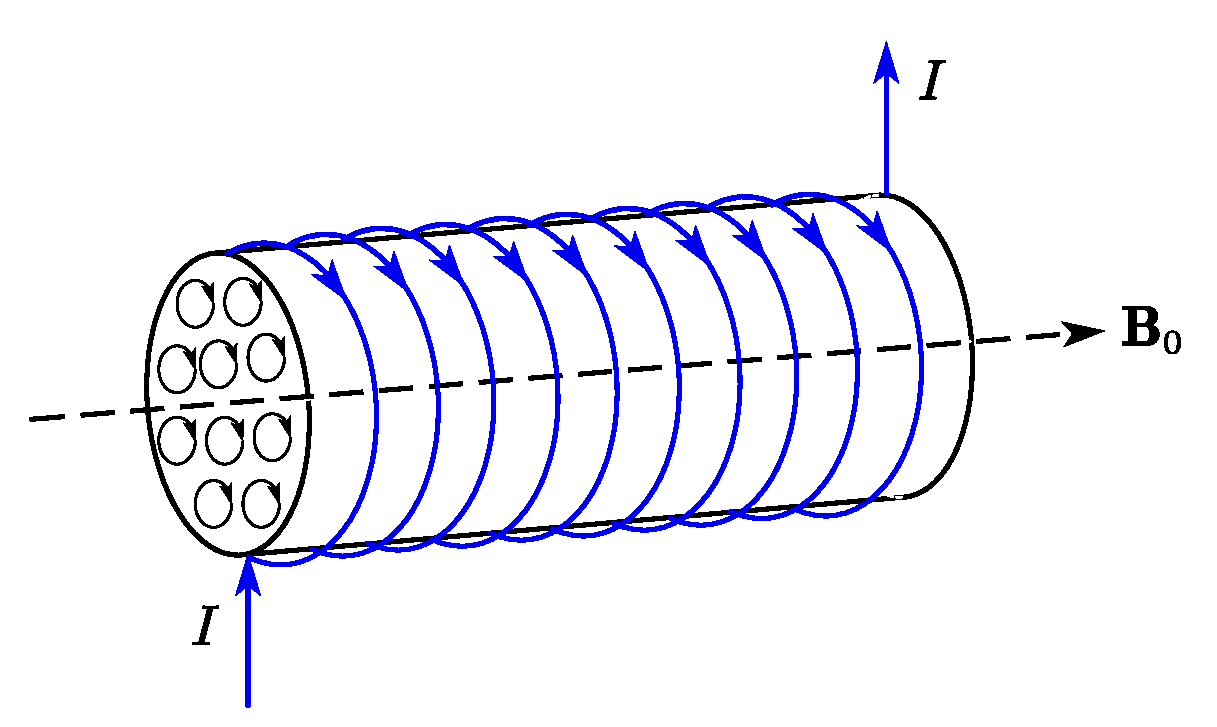
\includegraphics[width=10cm]{./figures/MaInte_1.pdf}
\caption{无限长的载流直螺线管} \label{MaInte_fig1}
\end{figure}
为简单起见,我们选一特例来讨论.设有一无限长的载流直螺线管,管内充满均匀磁介质,电流在螺线管内激发均匀磁场,如\autoref{MaInte_fig1} 所示.在此磁场中磁介质被均匀磁化,这时磁介质中各个分子电流平面将转到与磁场的方向相垂直.

\begin{figure}[ht]
\centering
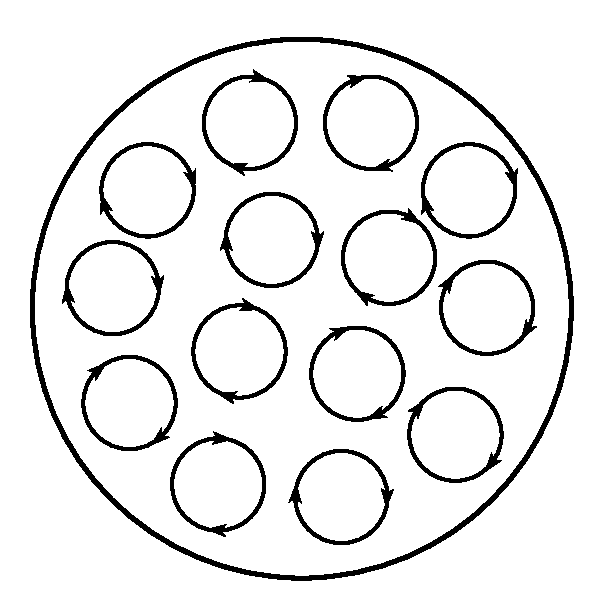
\includegraphics[width=5cm]{./figures/MaInte_3.pdf}
\caption{任一截面上分子电流排列} \label{MaInte_fig3}
\end{figure}
\begin{figure}[ht]
\centering
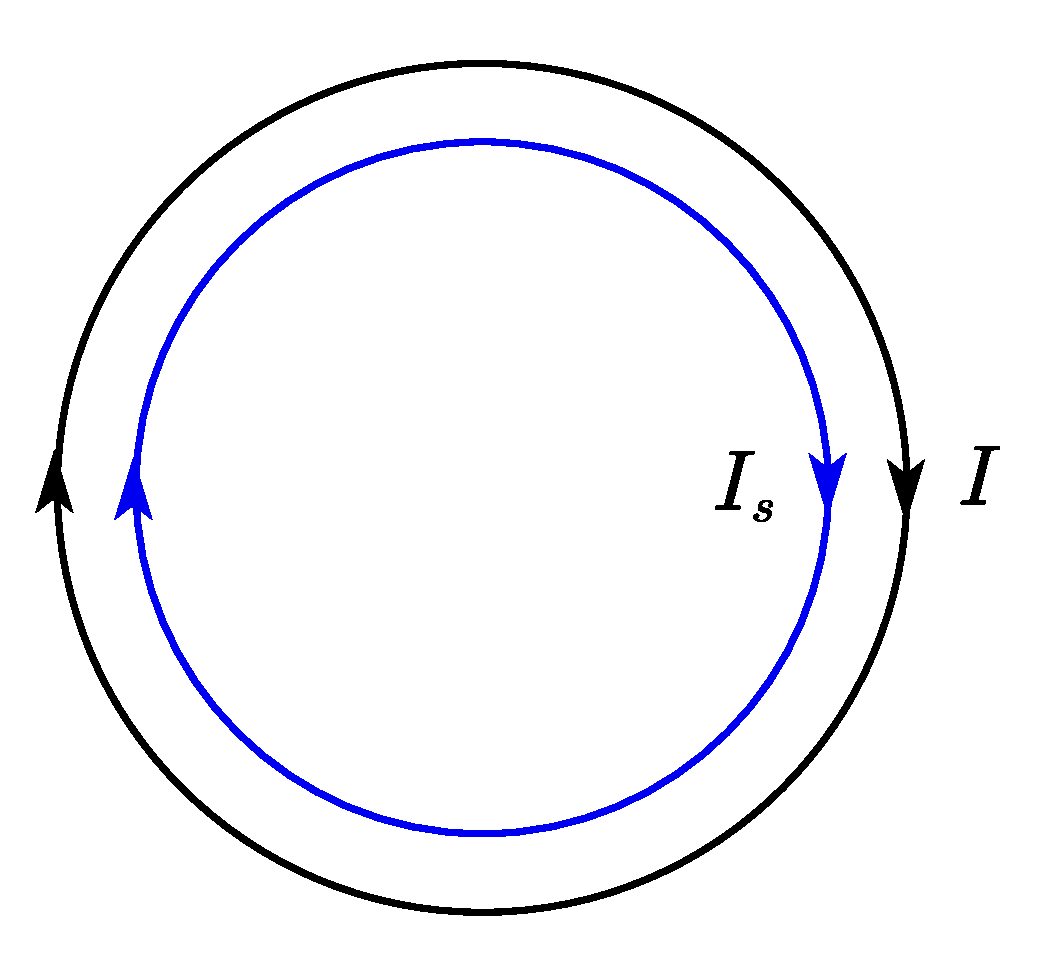
\includegraphics[width=5cm]{./figures/MaInte_4.pdf}
\caption{任一截面上分子电流排列} \label{MaInte_fig4}
\end{figure}
我们来看磁介质内任一截面上分子电流排列的情况.从\autoref{MaInte_fig3} 和\autoref{MaInte_fig4} 中可以看出,在磁介质内部任意一点处,总是有两个方向相反的分子电流通过,结果相且抵消;只有在截面边缘处,分子电流未被抵消,形成与截面边缘重合的圆电流.对磁介质的整体来说,未被抵消的分子电流是沿着柱面流动的,称为\textbf{安培表面电流}(或叫\textbf{磁化面电流}).对顺磁性物质,安培表面电流和螺线管上导线中的电流$I$方向相同;对抗磁性物质,则两者方向相反.我们上面的图中都是顺磁质的情况.设$q $为圆柱形磁介质表面上单位长度的磁化面电流,即磁化面屯流的线密度,$ S $为磁介质的截面积,$ l $为所选取的一段磁介质的长度.在$l $长度上,表面电流的总量值为$I_s=\alpha_sl$,因此在这段磁介质总体积$Sl$中的总磁矩为
\begin{equation}
\sum \mathbf{m}_{mole}=I_{s} \mathbf S=\alpha_{s} l \mathbf S
\end{equation}
按定义,$\mathbf  M $为单位体积内的磁矩,所以
\begin{equation}
M=\frac{\left|\sum \mathbf  m_{mole}\right|}{V}=\frac{\alpha_{s} S l}{S l}=\alpha_s
\end{equation}

即磁介质表面某处的磁化面电流线密度的大小等于该处磁化强度的量值.上述结果是从均匀磁介质被均匀磁化的特例导出的,在一般情况中,应该是磁介质表面上磁化面电流线密度应等于该处磁化强度的切线分量.而且在不均匀磁介质内部,由于排列着的分子电流未能相互抵消,此时磁体内各点都有磁化电流.

\begin{figure}[ht]
\centering
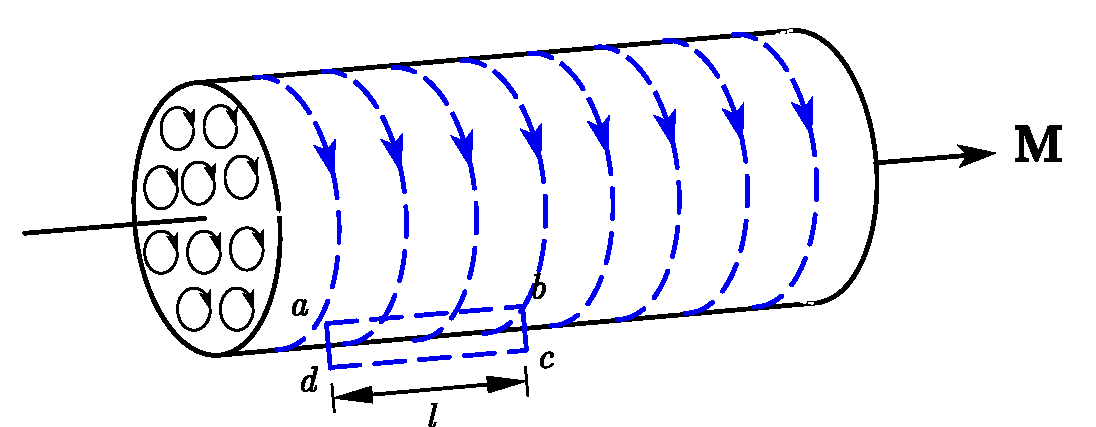
\includegraphics[width=8cm]{./figures/MaInte_2.pdf}
\caption{无限长的载流直螺线管} \label{MaInte_fig2}
\end{figure}
为了求得磁化电流与磁化强度的联系,我们来计算磁化强度对闭合回路的线积分$\displaystyle \oint \mathbf M \vdot \mathrm{d} \mathbf l$与磁化电流的关系.仍用前述特例,在\autoref{MaInte_fig2} 所示的圆柱形磁介质的边界附近,取一长方形闭合回路$abcd$,$ab $边在磁介质内部,它平行于柱体轴线,长度为$l$.而$bc$、$ad $两边则垂直于柱面在磁介质内部各点处,$\mathbf M$都沿$ab $方向,大小相等,在柱外各点处$\mathbf M=0$,所以$\mathbf M $沿$bc$、$cd$、$da $三边的积分为零,因而$\mathbf M $对闭合回路$abcd$的积分等于$\mathbf M $沿$ab $边的积分,即
\begin{equation}
\oint \mathbf{M}\vdot  \mathrm{d} \mathbf{l}=\int_{a}^{b} \mathbf{M} \vdot  \mathrm{d} \mathbf{l}=M|a b|=M l
\end{equation}
将$M=\alpha_s$, 代入后得
\begin{equation} \label{MaInte_eq1}
\oint \mathbf M \cdot \mathrm{d} l=\alpha_{s} l=I_{s}
\end{equation}
这里,$\alpha_sl=I_s$就是通过以闭合回路$abcd$为边界的任意曲面的总磁化电流,所以\autoref{MaInte_eq1} 表明\textbf{磁化强度对闭合回路的线积分等于通过回路所包围的面积内的总磁化电流}.\autoref{MaInte_eq1} 虽是从均匀磁化介质及长方形闭合回路的简单特例导出的,但却是在任何情况下都普遍适用的关系式.
